

\chapter{Mappings in Knowledge Graph Evolution}
\label{chapter:evolution}

Knowledge graphs are not immutable, as they along with the ontology or network of ontologies that defines their schema are subject to modifications. This need for evolution may triggered by changes in the domain of knowledge or on the graph consumption requirements in downstream tasks. 
An example is the need to add information about a triple, thus making statements about statements (i.e. statement reification).
%Reification is usually used to incorporate metadata and provenance to existing triples~\cite{frey2019evaluation}.
%Throughout the years, different representations have been proposed for reifying statements in RDF 
%, such as Named Graphs~\cite{carroll2005namedgraphs}, N-Ary Relationships~\cite{naryw3c2006} or RDF-star~\cite{hartig2017foundations}. 
For instance, Nanopublications~\parencite{groth2010nanopubs} adopt a Named Graph-based~\parencite{carroll2005namedgraphs} model to publish minimal scientific statements along with their provenance and associated context. Meanwhile, in ontology engineering, N-Ary Relationships~\parencite{naryw3c2006} are widely used as an ontology design pattern~\parencite{gangemi2013multi}. Moreover, the well-known knowledge base of Wikidata has implemented its own reification schema based on \textit{qualifiers}~\parencite{erxleben2014introducing}. 

It is not uncommon for an existing KG to strive for adopting one of these representations. Several studies throughout the years prove that these different representations impact the downstream KG consumption tasks; for query performance~\parencite{das2014tale,nguyen2014don,alocci2015property,hernandez2015reifying,frey2019evaluation,orlandi2021benchmarking} as well as for human consumption and machine learning-based tasks~\parencite{iglesias2023kgconsumption}. Some examples of existing KGs that have changed their representation include the preliminar transition of Wikidata to the current qualifier-based representation~\parencite{erxleben2014introducing}; the publication of the DisGeNet KG as Nanopublications~\parencite{queralt2016disgenet}, and the introduction of RDF-star in the European Agency of Railway  KG\footnote{\url{https://data-interop.era.europa.eu/}}.

When the situation comes that a re-structuration of the knowledge graph is needed, the following question arises: Which is more convenient, to construct the graph from the original input data sources again, or to re-construct it within the triplestore? This section analyses which of these approaches reports better performance and the parameters that influence the choice. 
To this end, we perform a comprehensive empirical study of this transformation in four representations (Standard Reification, N-Ary Relationships, Named Graphs and RDF-star) using (i) declarative mapping languages to construct each representation with KG construction engines and (ii) transformation per peers of representations with SPARQL \texttt{CONSTRUCT} queries in different triplestores. This section aims to unravel the aspects to consider when re-constructing a knowledge graph, to help in the decision on how to perform it and assess the role that mapping technologies can play in this kind of KG evolution. %We also raise awareness of recently overlooked aspects of \texttt{CONSTRUCT} queries, while contributing to research on the impact of RDF reification to enhance KG management.


\section{Motivation}
\label{sec:chp6-1_mot-example}

\subsection{KG Representation impact on its consumption}

Previous studies comparing knowledge representations have focused primarily on query performance~\citep{das2014tale,nguyen2014don,alocci2015property,hernandez2015reifying,frey2019evaluation,orlandi2021benchmarking} and graph interoperability~\citep{angles2019rdf,angles2020mapping}. For this scenario, the representations need to ensure efficiency to minimize performance time. 
However, applications relating to exploration by end users and machine learning over KGs have not been taken into account~\citep{karger2014semantic,hogan2020twodecades}. 
Knowledge exploration scenarios, e.g., browsing, are impacted by representational choices, and therefore the selected representations should reduce the cognitive load and user expertise needed to explore, access, and acquire knowledge.
Similarly, many embedding models-based tasks such as knowledge graph completion~\citep{ren2022smore} require adequate representations to maximize the performance of the models on downstream predictive tasks.

Motivated by the lack of research on the representation impact on a broader set of KG consumption tasks, we carry out in \cite{iglesias2023kgconsumption} an evaluation to assess the fitness of four popular KR approaches (Standard Reification, N-Ary Relationships, Wikidata qualifiers, and RDF-Star) for the needs of the abovementioned scenarios. 
First, to understand user preferences in knowledge exploration tasks, we run a user study where participants interact with a web browser interface and a query endpoint to determine the representation that improves knowledge acquisition for real-world questions.
Then, to assess the differential performance of the representations, we test several queries using synthetic and real-world data.
Lastly, to estimate the impact on KG embedding model performance, we train and evaluate a selection of these models for the KG completion task with different representations.

\begin{table}[t]
    \centering
    \caption[Summary results of the representation impact on KG consumption scenarios]{Summary of the fitness for each representation evaluated in the studied scenarios, where \checkmark means suitable, $\backsim$ is acceptable, X is avoidable and * indicates that the value is not tested but equivalent to Qualifiers.}
    \label{tab:chp6-1_kgconsumption_summary}
    \resizebox{0.9\columnwidth}{!}{\begin{tabular}{ccccc}
          & \begin{tabular}[c]{@{}c@{}}\textbf{User}\\\textbf{interaction}\end{tabular} & \begin{tabular}[c]{@{}c@{}}\textbf{Simple graphs}\\\textbf{and queries}\end{tabular} & \begin{tabular}[c]{@{}c@{}}\textbf{Large graphs and}\\\textbf{demanding queries}\end{tabular} & \begin{tabular}[c]{@{}c@{}}\textbf{Graph}\\\textbf{completion}\end{tabular} \\ \midrule
        \textbf{Qualifiers} & \checkmark & \checkmark & \checkmark & \checkmark (RotatE) \\ \midrule
        \textbf{RDF-star} & \checkmark* & \checkmark & $\backsim$ & -\\ \midrule
        \textbf{N-Ary Rel.} & \checkmark & \checkmark & $\backsim$ & \checkmark (TransE) \\ \midrule
        \textbf{Std. Reif.} & X & \checkmark & $\backsim$ & \checkmark (ComplEx) \\ \bottomrule
    \end{tabular}}
\end{table}

This study found significant differences for particular scenarios, summarized in \cref{tab:chp6-1_kgconsumption_summary}, drawing the following conclusions: 
\begin{enumerate}
    \item Standard Reification is the least suitable for users. Its anti-intuitive structure results time-consuming to navigate with, and it introduces additional complexity to retrieve correct and complete information.
    \item RDF-star still needs improved support in all studies scenarios, as it is underway of becoming part of the RDF 1.2 specification~\cite{hartig2023rdf}. At the moment, it is risky to use it in high-demanding scenarios.
    \item Qualifiers obtain steadily better results for retrieving results in high-demanding querying scenarios. Despite being restricted to Wikidata at the moment, its representation could be considered to be adopted in more knowledge graphs.
    \item Analysing and understanding how each embedding model works is key to select a representation for graph completion (and hence, additional embedding-based tasks). While for the other scenarios all representations showed acceptable behaviour, here the decision is critical.
    \item Promoting the use of interfaces such as browsers highly improves the user experience in knowledge exploration. These interfaces help mask the representation complexity and differences, which directly influences the adoption and usability of semantic resources, an aspect usually overlooked.
\end{enumerate}

Overall, the lack of a good-for-all solution raises the need of improving the interoperability among representations, especially in cases where knowledge graphs are consumed for very different purposes.



\subsection{Re-construction example}

\begin{figure}[t!]
    \centering
    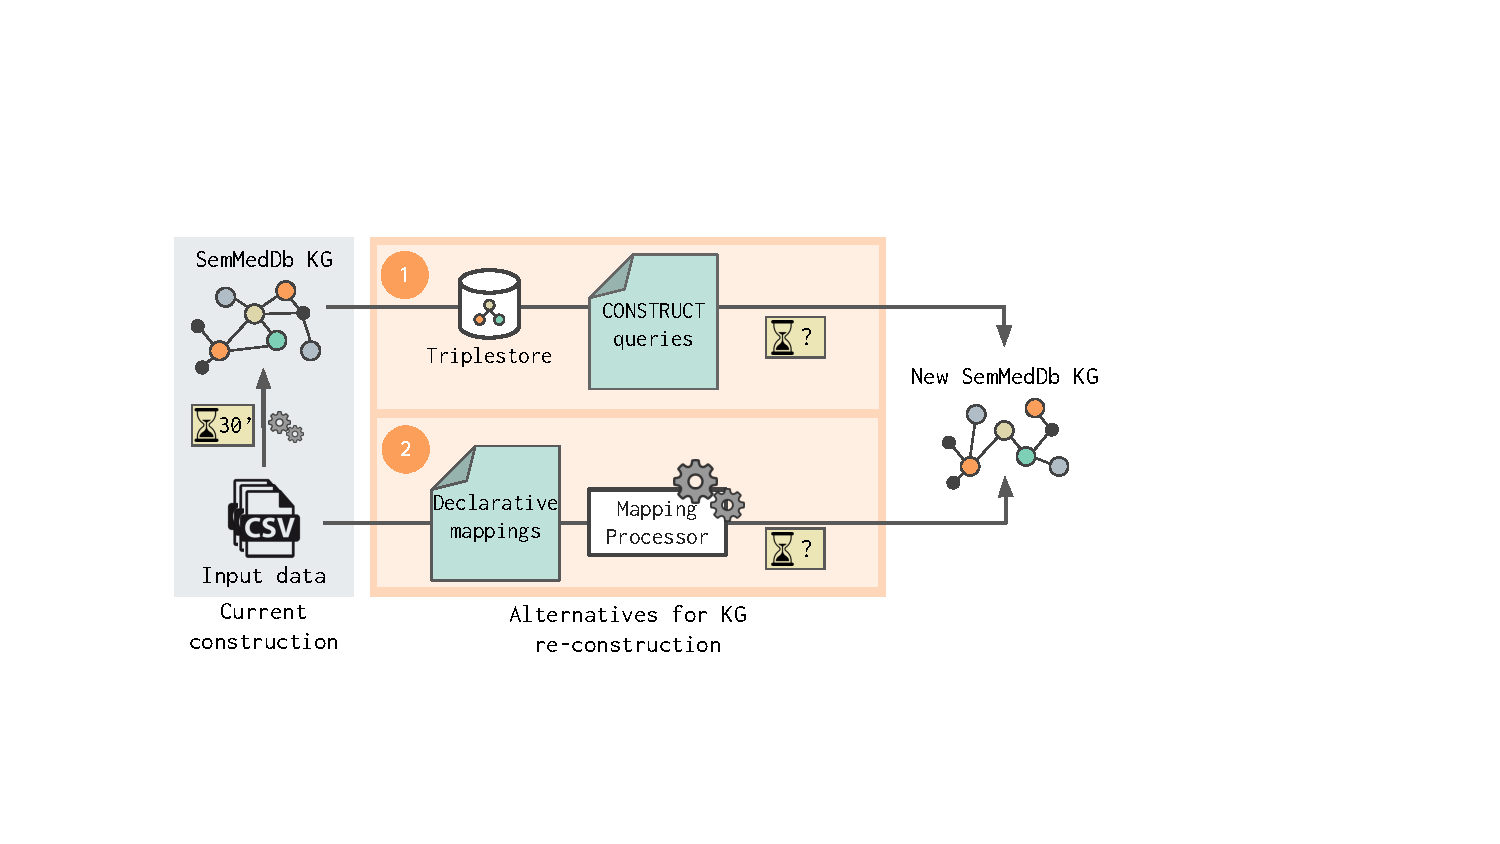
\includegraphics[width=1\linewidth]{figures/chp6-1_motivating-example.pdf}
    \caption[KG re-construcion alternatives]{Alternatives for re-constructing a pre-existing knowledge graph.}
    \label{fig:chp6-1_mot-example}
\end{figure}

Consider the SemMedDB dataset, that contains entities extracted from biomedical texts, as well as the semantic types of these concepts and a timestamp of when they were extracted. A stable version of a knowledge graph represents this information, where the timestamp and semantic type are related to its correspondent entity with an N-Ary relationship. However, the maintainers of this knowledge graph want to reduce the size of the graph by reducing the number of nodes, as well as to represent this information with RDF-star to start adopting the RDF 1.2 specification.

The graph maintainers have access to the original source data, so they can change the original KG construction pipeline, that uses declarative mappings to construct the graph. However, since this graph is not going to be updated with new data, it is also possible to change the structure of the graph with queries within the triplestore where it is maintained. They know the time it takes to generate the graph in its original representation. However, they are not certain whether generating the graph in the new representation using this pipeline will take more time, or if with queries the transformation could be performed faster (\cref{fig:chp6-1_mot-example}). Hence, the objective of this work consist of assessing the aspects that influence this situation to help in making an informed decision.


\section{Methodology}
\label{sec:chp6-1_methodology}

In this section we present the methodology followed to analyze the impact of different approaches for re-constructing knowledge graphs from a reification perspective. More in detail, we compare two ways of re-structuring a KG to change its reification approach, (i) with declarative mapping technologies from scratch (e.g., RML~\citep{Dimou2014rml,iglesias2023rml}) and (ii) with \texttt{CONSTRUCT} queries in a triplestore from the previous version of the graph. We aim to answer the following research questions: \ana{ojo a esto para cuando estén los objetivos y demás escritos }
\textbf{(RQ1)} In which cases is it more efficient in terms of time to either construct a reified knowledge graph from the original data sources or to re-construct it within a triplestore?
\textbf{(RQ2)} Which of these two approaches is more scalable as the size of the data increases?
\textbf{(RQ3)} What is the impact of the different reification representations on triplestores and mapping processors?
%In this section, we describe the experimental configuration for the evaluation carried out to answer these research questions. 
All resources to reproduce the experiments are available on GitHub.\footnote{\url{https://github.com/oeg-upm/kg-reconstruction-eval}}



\subsection{Dataset}
\label{sec:chp6-1_dataset}

\ana{ojo que esta sección es como para la de rml-star}

We use the Semantic MEDLINE Database (SemMedDB)~\citep{SemMedDB} in the experimental evaluation. This database consists of a repository with biomedical entities and relationships (subject-predicate-object) extracted from biomedical texts.
%, mainly titles and abstracts from PubMed citations. 
This dataset is available as a relational database and CSV files.\footnote{\url{https://lhncbc.nlm.nih.gov/ii/tools/SemRep\_SemMedDB\_SKR/SemMedDB\_down\-load.html}}
It is licensed under the UMLS - Metathesaurus License Agreement,\footnote{\url{https://www.nlm.nih.gov/research/umls/knowledge\_sources/metathesaurus/release\-/license\_agreement.html}} which does not allow its distribution, but it may be accessed with an account with the UMLS license.\footnote{An account with the UMLS license can be requested at \url{https://www.nlm.nih.gov/databases/umls.html}.}


We use the CSV files for (i)~\textit{entity} predictions (from ENTITY.csv), and (ii)~\textit{predication} predictions (from PREDICATION.csv and PREDICATION\_AU\-X.csv). Listings~\ref{lst:chp6-1_semmeddb_entity},~\ref{lst:chp6-1_semmeddb_pred} and~\ref{lst:chp6-1_semmeddb_predaux} illustrate the columns used from the files with synthetic data.
For \textit{predications}, only data for \textit{subjects} is shown; the missing columns regarding \textit{objects} follow the same structure as \textit{subjects}.
%This data contains information on predicted entities and predicted subject-predicate-object predications.
\textit{Subjects} and \textit{objects} (from \textit{predications}), and \textit{entities} are assigned a \textit{semantic type} with a confidence score.
These \textit{semantic types} categorize the extracted concept in the biomedical domain.\footnote{\url{https://www.nlm.nih.gov/research/umls/new\_users/online\_learning/SEM\_003.html}}
In addition, the extraction of \textit{subjects} and \textit{objects} is assigned a timestamp on when it took place. 
Thus, the score and timestamp represent metadata about other statements, which are fit to represent using reification.

We model this tabular dataset as five annotated statements: 
Three assign \textit{semantic types} to \textit{subjects}, \textit{objects}, and \textit{entities} with a confidence score; and two provide the timestamp for the extraction of \textit{subjects} and \textit{objects} from text.  


\noindent\begin{minipage}{0.42\linewidth}
\begin{captionedlisting}{lst:chp6-1_semmeddb_entity}{ENTITY.csv snippet.}
\centering
\begin{tabular}{c}
\hspace{-0.7em}
{
\begin{lstlisting}[basicstyle=\ttfamily\small,label={lst:chp6-1_semmeddb_entity},columns=flexible]
ENTITY_ID , SEMTYPE , SCORE
12345      , orga     , 790
\end{lstlisting}
}
\end{tabular}
\end{captionedlisting}
\end{minipage}
\,\,\,\,\hfill
\begin{minipage}{0.58\linewidth}
\begin{captionedlisting}{lst:chp6-1_semmeddb_pred}{PREDICATION.csv snippet.}
\centering
\begin{tabular}{c}
\hspace{-1em}
{
\begin{lstlisting}[basicstyle=\ttfamily\small,label={lst:chp6-1_semmeddb_pred},columns=flexible]
PREDICATION_ID , SUBJ_SEMTYPE , SUBJ_NAME
13579            , Semtype       , SubjName
\end{lstlisting}
}
\end{tabular}
\end{captionedlisting}
\end{minipage}

\noindent\hspace{0.23\linewidth}\begin{minipage}{\linewidth}
\begin{captionedlisting}{lst:chp6-1_semmeddb_predaux}{PREDICATION\_AUX.csv snippet.}
\centering
\begin{tabular}{c}
\hspace{-7em}
{
\begin{lstlisting}[basicstyle=\ttfamily\small,label={lst:chp6-1_semmeddb_predaux},columns=flexible]
PREDICATION_AUX_ID , PREDICATION_ID , SUBJ_SCORE , TIMESTAMP
67890                , 13579            , 800         , 1651740766
\end{lstlisting}
}
\end{tabular}
\end{captionedlisting}
\end{minipage}


To test the scalability of the evaluated approaches, we subset this dataset into four sizes taking as input from the abovementioned CSV files with (i)~1K rows, (ii)~10K rows, (iii)~100K rows and (iv)~1M rows. The number of triples produced for each reification version in each scale is shown in \cref{tab:chp6-1_data-triple-number}.

\begin{table}[t]
\caption[SemMedDB scale sizes]{Number of triples of the SemMedDB graph in the selected representations for each scale.}
\label{tab:chp6-1_data-triple-number}
\centering
\begin{tabular}{cccccc}
    \cmidrule{2-6}
    & & \textbf{1K} & \textbf{10K} & \textbf{100K} & \textbf{1M} \\ \midrule
    \textbf{Standard Reification} & & 25,000 & 249,997 & 2,499,966 & 24,999,607 \\ \midrule
    \textbf{Named Graphs} & & 10,000 & 99,994 & 999,932 & 9,999,190 \\ \midrule
    \textbf{N-Ary Relationships} & & 15,000 & 149,997 & 1,499,966 & 14,999,595 \\ \midrule
    \textbf{RDF-star} & & 8,485 & 78,655 & 710,588 & 6,503,388 \\ \bottomrule
\end{tabular}
\end{table}




\subsection{Mappings and Queries}
\label{sec:chp6-1_map-queries}
The following resources are used: 
(i)~a set of declarative mappings that are used for constructing the knowledge graph from the SemMedDB tabular files in the four selected reification representations; and (ii)~a set of SPARQL queries that are used for re-constructing the graph within different triplestores. A summary of their characteristics is shown in \cref{tab:chp6-1_mapping-char}.

We use two sets of mappings, one set written in the RML mapping language~\citep{iglesias2023rml}, and the other in SPARQL-Anything~\citep{asprino2023sparql-anything}. These languages allow describing transformation of heterogeneous data sources into RDF following the schema provided by an ontology or vocabulary, and are processed by different engines (see \cref{sec:chp6-1_engines}). Each set of mappings is comprised of four mappings, to construct the knowledge graphs in the four representations selected (i.e. Standard Reification, N-Ary Relationships, Named Graphs and RDF-star).


RML extends the R2RML Recommendation~\citep{das2012r2rml} to describe more data sources besides Relational Databases. RML rules are grouped within \textit{Triples Maps}, which contain one \textit{Logical Source}, one \textit{Subject Map} and zero to multiple \textit{Predicate Object Maps}. \textit{Logical Sources} describe the input data to be transformed. \textit{Subject Maps} indicates how the subjects of the triples are created, while \textit{Predicate Object Maps} specify how the predicates and objects of the triples are created. \cref{lst:chp6-1_rml-star} shows an example of a mapping that generates in RDF-star the annotation of the semantic types of \textit{entities} with a score from the CSV file shown in \cref{lst:chp6-1_semmeddb_entity}. This mapping uses the RML-star module~\citep{delva2021rml-star,iglesias2023rml} to generate RDF-star graphs, which allows RML to quote \textit{Triples Map} with the \texttt{rml:quotedTriplesMap} property. For these mappings, we show the number of sets of rules (i.e. \textit{Triples Map}) and  \textit{Predicate Object Maps} specified (\cref{tab:chp6-1_mapping-char}).

\noindent\begin{minipage}{1\linewidth}
\begin{captionedlisting}{lst:chp6-1_rml-star}{RML-star mapping snippet to create the RDF-star graph for \textit{entity} from data in \cref{lst:chp6-1_semmeddb_entity}. }
\centering
\begin{tabular}{cc}
{\begin{lstlisting}[basicstyle=\ttfamily\small,label={list:example1}]
<#Entity> 
 a rml:TriplesMap ;
 rml:logicalSource [
  rml:source "ENTITY.csv"
 ];
 rml:subjectMap [
  rml:template ":{ENTITY_ID}"
 ];
 rml:predicateObjectMap [
  rml:predicate :semanticType;
  rml:objectMap [
   rml:reference "SEMTYPE"
  ] ] .
\end{lstlisting}}
&
%\hspace{3em}
{\begin{lstlisting}[basicstyle=\ttfamily\small,label={list:example1},numbers=right,firstnumber=13]
<#EntityScore> 
  a rml:AssertedTriplesMap ;
 rml:logicalSource [
  rml:source "ENTITY.csv"
 ];
 rml:subjectMap [
  rml:quotedTriplesMap <#Entity>;
 ];
 rml:predicateObjectMap [
  rml:predicate :score ;
  rml:objectMap [
   rml:reference "SCORE"
  ] ] .
\end{lstlisting}}

\end{tabular}
\end{captionedlisting}
\end{minipage}


\begin{table}[t!]
    \caption[Characteristics of evaluation mapping]{Characteristics of mappings in RML and SPARQL-Anything. \#TM stands for number of Triples Map, \#POM for Predicate Object Map, and \#TP for Triple Patterns. The shown operators appear usually in the \texttt{WHERE} clause; the ones marked with $^c$ appear in the \texttt{CONSTRUCT} clause. }
    \label{tab:chp6-1_mapping-char}
    \centering
    \begin{tabular}{ccc|cc}
        \cmidrule{2-5}
         & \multicolumn{2}{c|}{\textbf{RML}} & \multicolumn{2}{c}{\textbf{SPARQL-Anything}}  \\ \midrule
         & \textbf{\#TM} & \textbf{\#POM} & \textbf{\#TP$^c$} & \textbf{Additional operators}  \\ \midrule
         \textbf{Standard Reification} & 9 & 20 & 25 & UNION, BIND  \\ \midrule
         \textbf{Named Graphs} & 10 & 10 & 10 & UNION, BIND, GRAPH$^c$  \\ \midrule
         \textbf{N-Ary Relationships} & 13 & 15 & 15 & UNION, BIND  \\ \midrule
         \textbf{RDF-star} & 10 & 10 & 10 & UNION, BIND  \\  \midrule
         
    \end{tabular}
\end{table}

SPARQL-Anything heavily relies on the SPARQL syntax, overriding the \texttt{SERVICE} operator while leveraging the rest of its features. This operator is then always present in the queries and hence is not shown in the table. The graphs are built with \texttt{CONSTRUCT} clauses. \cref{lst:chp6-1_sparql-anything} shows a mapping example that generates in RDF-star the annotation of the semantic types of \textit{entities} with a score from the CSV file shown in \cref{lst:chp6-1_semmeddb_entity}.
For each mapping, we show the number of triple patterns in this clause and additional SPARQL clauses (\cref{tab:chp6-1_mapping-char}). All mappings contain the same number of triple patterns in the \texttt{WHERE} clause.




\noindent\begin{captionedlisting}{lst:chp6-1_sparql-anything}{SPARQL-Anything mapping snippet to create the RDF-star graph for \textit{entity} from data in \cref{lst:chp6-1_semmeddb_entity}.  }
\centering
{
\begin{lstlisting}[basicstyle=\ttfamily\small,label={list:example1},columns=flexible,language=sparql]
CONSTRUCT {
  ?entity_id_iri :semanticType ?entity_semtype .
  << ?entity_id_iri :semanticType ?entity_semtype >> :score ?entity_score .
 } WHERE {
  {  SERVICE <x-sparql-anything:location=./data/entity.csv>
   { [] xyz:ENTITY_ID ?entity_id;
     xyz:SEMTYPE ?entity_semtype;
     xyz:SCORE ?entity_score;
    BIND(uri(concat(str("http://semmeddb.com/entity/"),
                        encode_for_uri(?entity_id))) as ?entity_id_iri)
   }  } }

\end{lstlisting}
}
\end{captionedlisting}



SPARQL queries use the \texttt{CONSTRUCT} clause to re-construct a given graph represented with one of the reifications into the other three representations. We use twelve queries to transform all pairs of representations, whose characteristics are shown in \cref{tab:chp6-1_query-char}. We show for each query the number of triple patterns in the \texttt{WHERE} and \texttt{CONSTRUCT} clauses, and the additional operators used. Except for \texttt{GRAPH}, the rest of operators only appear within the \texttt{WHERE} clause. An example of a query is shown in \cref{lst:chp6-1_sparql-construct}, which generates RDF-star from Named graphs.


\noindent\begin{captionedlisting}{lst:chp6-1_sparql-construct}{SPARQL query snippet to create the RDF-star graph from the Named Graphs representation for \textit{entity}. }
\centering
{
\begin{lstlisting}[basicstyle=\ttfamily\small,label={list:example1},columns=flexible,language=sparql]
CONSTRUCT  {
  ?entity_id_iri :semanticType ?entity_semtype .
  << ?entity_id_iri :semanticType ?entity_semtype >> :score ?entity_score .
} WHERE {
  GRAPH ?entity_graph_iri { ?entity_id_iri :semanticType ?entity_semtype }
  ?entity_graph_iri :score ?entity_score . 
}
\end{lstlisting}
}
\end{captionedlisting}



\begin{table}[t!]
\caption[Characteristics of evaluation SPARQL queries]{Characteristics of the SPARQL queries used for the evaluation to transform the graph from a \textit{source} representation to a \textit{target} representation. \#TP stands for the number of triple patterns. Fields marked with $^c$ appear in the \texttt{CONSTRUCT} clause, while $^w$ indicates the \texttt{WHERE} clause. }
\centering
\label{tab:chp6-1_query-char}
\resizebox{\columnwidth}{!}
{\begin{tabular}{cccccccccc}
    \cmidrule{2-10}
 & \textbf{Source} & \textbf{Target} & \textbf{\#TP$^w$} & \textbf{\#TP$^c$} & \textbf{UNION$^w$} & \textbf{BIND$^w$} & \textbf{FILTER$^w$} & \textbf{VALUES$^w$} & \textbf{GRAPH}  \\ \midrule
\textbf{Q1} & \multirow{4}{*}{\textbf{N-AryRel.}} & \textbf{Std. Reif.} & 6 & 10 & \checkmark &  &  & \checkmark &  \\ \cmidrule{3-10}
 \textbf{Q2} & & \textbf{RDF-Star} & 6 & 4 & \checkmark &  &  & \checkmark &  \\ \cmidrule{3-10}
 \textbf{Q3} & & \textbf{Named Graphs} & 6 & 4 & \checkmark &  &  & \checkmark & \checkmark $^c$ \\ \midrule
\textbf{Q4} & \multirow{4}{*}{\textbf{Std. Reif.}} & \textbf{RDF-star} & 8 & 4 & \checkmark &  &  & \checkmark &  \\ \cmidrule{3-10}
 \textbf{Q5} & & \textbf{N-Ary Rel.} & 20 & 15 & \checkmark &  & \checkmark &  &  \\ \cmidrule{3-10}
 \textbf{Q6} & & \textbf{Named Graphs} & 8 & 4 & \checkmark &  &  & \checkmark & \checkmark $^c$ \\ \midrule
\textbf{Q7} & \multirow{4}{*}{\textbf{RDF-star}} & \textbf{Std. Reif.} & 5 & 25 & \checkmark & \checkmark & \checkmark &  &  \\ \cmidrule{3-10}
 \textbf{Q8} & & \textbf{N-Ary Rel.} & 5 & 15 & \checkmark & \checkmark & \checkmark &  & \\ \cmidrule{3-10}
 \textbf{Q9} & & \textbf{Named Graphs} & 5 & 10 & \checkmark & \checkmark & \checkmark &  & \checkmark $^c$ \\ \midrule
\textbf{Q10} & \multirow{4}{*}{\textbf{Named Graphs}} & \textbf{Std. Reif.} & 4 & 10 & \checkmark &  &  & \checkmark & \checkmark $^w$ \\ \cmidrule{3-10}
 \textbf{Q11} & & \textbf{RDF-Star} & 4 & 4 & \checkmark &  &  & \checkmark & \checkmark $^w$ \\ \cmidrule{3-10}
 \textbf{Q12} & & \textbf{N-Ary Rel.} & 4 & 15 & \checkmark &  &  & \checkmark & \checkmark $^w$  \\  \bottomrule
\end{tabular}}
\end{table}



\subsection{Engines}
\label{sec:chp6-1_engines}
We choose a set of 2 mapping processors and 3 triplestores to be representative in our evaluation, while focusing on open-source tools. The selected mapping processors, Morph-KGC (v2.5.0)~\citep{arenas2022morphkgc} and SPARQL-Anything (v0.8.1)~\citep{asprino2023sparql-anything} are the systems with a stable version capable of producing RDF-star at the time of writing this paper. The SDM-RDFizer~\citep{iglesias2020rdfizer} is in the process of implementing this feature, but no stable version has been released yet. Regarding triplestores, we use the free version of GraphDB (v10.2.1), and the open-source Jena Fuseki (v4.8.0) and Oxigraph (v0.3.16). While GraphDB and Jena Fuseki store the graph in physical memory, Oxigraph performs the queries in memory. All engines perform duplicate removal in the results by default, with the exception of Oxigraph. For this triplestore, we add and measure a second step of duplicate removal with BASH commands.


We did attempts to include Virtuoso in the evaluation; however, several issues raised. The number of queries this triplestore can perform is very limited in this evaluation (only 4 from 12): This triplestore
does not implement RDF-star yet, and cannot produce named graphs declared inside the \texttt{CONSTRUCT} clause. In addition, Virtuoso limits the number of triples that can be produced with this clause to 1M.\footnote{\url{https://lig-membres.imag.fr/rousset/publis/tess.pdf}} When this limit is removed, an error appears that impedes the writing of the result in a file when it is large, which has been unsolved for years.\footnote{\url{https://github.com/openlink/virtuoso-opensource/issues/11}} 




\subsection{Experimental setup and Metrics}
\label{sec:chp6-1_exp-setup}
We perform the evaluation in two steps. First, the KG construction system evaluation is run, taking as input the SemMedDb dataset in CSV format and the mappings, and producing the corresponding RDF datasets in the four selected representations. Then, the triplestore evaluation is carried out, taking as input the produced datasets in the KG construction system evaluation, and producing RDF datasets in another representation.


We measure the \textit{materialization time} to construct the RDF graph from the input data sources in KG construction systems.
For triplestores, we measure \textit{query execution time} as the total time from query execution until the complete answer is generated. 
We also report the geometric mean of all queries that generate the same reified RDF graph, similar to previously used by~\citep{morsey2011dbpedia,schmidt2009sp}. 
The \textit{geometric mean} reports the central tendency of all execution times for a set of queries, reducing the effect of outliers. 
With this metric, we provide a general measurement of the performance of each triplestore when generating graphs in each representation. 
This allows an easier comparison with the KG construction systems. 
We run every experiment 5 times with a timeout of 24h, measure the time and calculate the median.
We run all experiments over an Ubuntu 20.04 server with
32 cores Intel(R) Xeon(R) Gold 5218R CPU @ 2.10GHz
102400 Mb RAM RDIMM, 3200 MT/s and 
100 Gb HD SSD 6 Gb/s. 




\section{Results}
\label{sec:chp6-1_results}


\begin{figure}[t!]
    \centering
    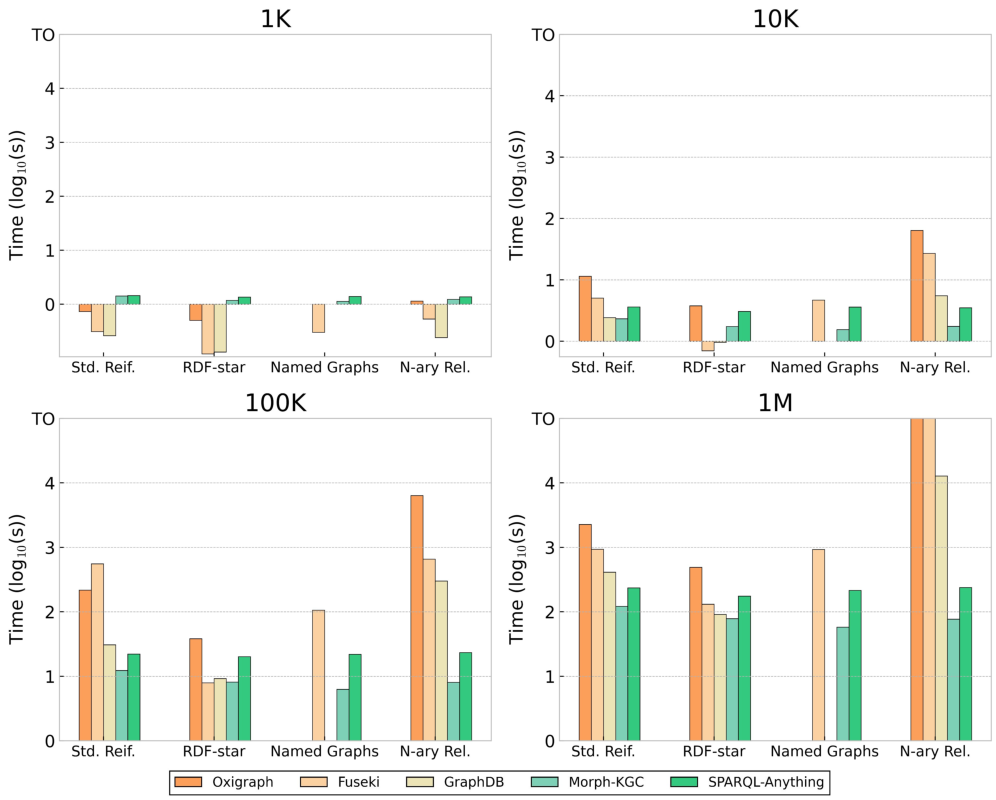
\includegraphics[width=\linewidth]{figures/chp6-1_results-map-queries.pdf}
    \caption[Overall execution times of KG re-construction evaluation]{Execution time for KG construction engines with declarative mappings, and triplestores with SPARQL queries. The results for the triplestores are grouped by the \textit{target} representation.}
    \label{fig:chp6-1_map-queries}
\end{figure}




The results of the evaluation performance are shown in Figs. \ref{fig:chp6-1_map-queries} and \ref{fig:chp6-1_queries}. \cref{fig:chp6-1_map-queries} reports the comparison between knowledge graph construction systems using declarative mappings, and triplestores with SPARQL queries. For the latter, the geometric mean of the query execution time for all queries that generate each representation is provided. \cref{fig:chp6-1_queries} reports a fine-grained comparison of the performance of each triplestore on the proposed queries that perform translations between each combination of pairs of representations.

Focusing on the comparison between triplestores and KG construction systems (\cref{fig:chp6-1_map-queries}), we generally observe that for small data sizes, triplestores obtain better results, while KG construction systems scale better as data size increases. However, in the case of producing RDF-star, Fuseki and GraphDB are competitive w.r.t. SPARQL-Anything or Morph-KGC. These triplestores obtain better results for the scales 1K and 10K, and similar ones for 100K and 1M. Additionally, despite the variety in mapping characteristics, neither Morph-KGC nor SPARQL-Anything seem to be highly affected by the different representations, as opposed to the triplestores. The differences are not remarkable, but in general Morph-KGC generates the fastest Names Graphs, in contrast with SPARQL-Anything, which performs better with RDF-star. For triplestores, producing N-Ary Relationships and Standard Reification is more costly than the other representations. Another relevant point to consider is that SPARQL 1.1 does not allow \texttt{GRAPH} clause within the \texttt{CONSTRUCT} operator. Thus, only Fuseki, which implements this extension natively, can generate the Named Graphs datasets.

Comparing the behavior of engines that perform the same task, GraphDB overcomes Fuseki and Oxigraph for SPARQL queries, while Morph-KGC reports better results than SPARQL-Anything for KG construction from heterogeneous data sources, as was reported in previous works~\citep{arenas2023morphstar}.
For small data sizes, GraphDB and Fuseki perform similar, while Oxigraph reports higher query execution time. This is because Oxigraph loads the complete RDF graph in memory and the physical data structures from Fuseki and GraphDB speed up query execution time. In larger datasets, GraphDB generally scales better than Fuseki, which for example, reports a timeout for generating N-Ary Rel. in scale 1M. 

%Answering the research questions, we can say that triplestores perform faster for small sizes (\textbf{RQ1}), while KG construction systems present a more robust behaviour with increasing data size (\textbf{RQ2}). In addition, triplestores are more influenced by the changes in representations, whereas KG construction systems are mostly unaffected (\textbf{RQ3}).

 


\begin{figure}[t!]
    \centering
    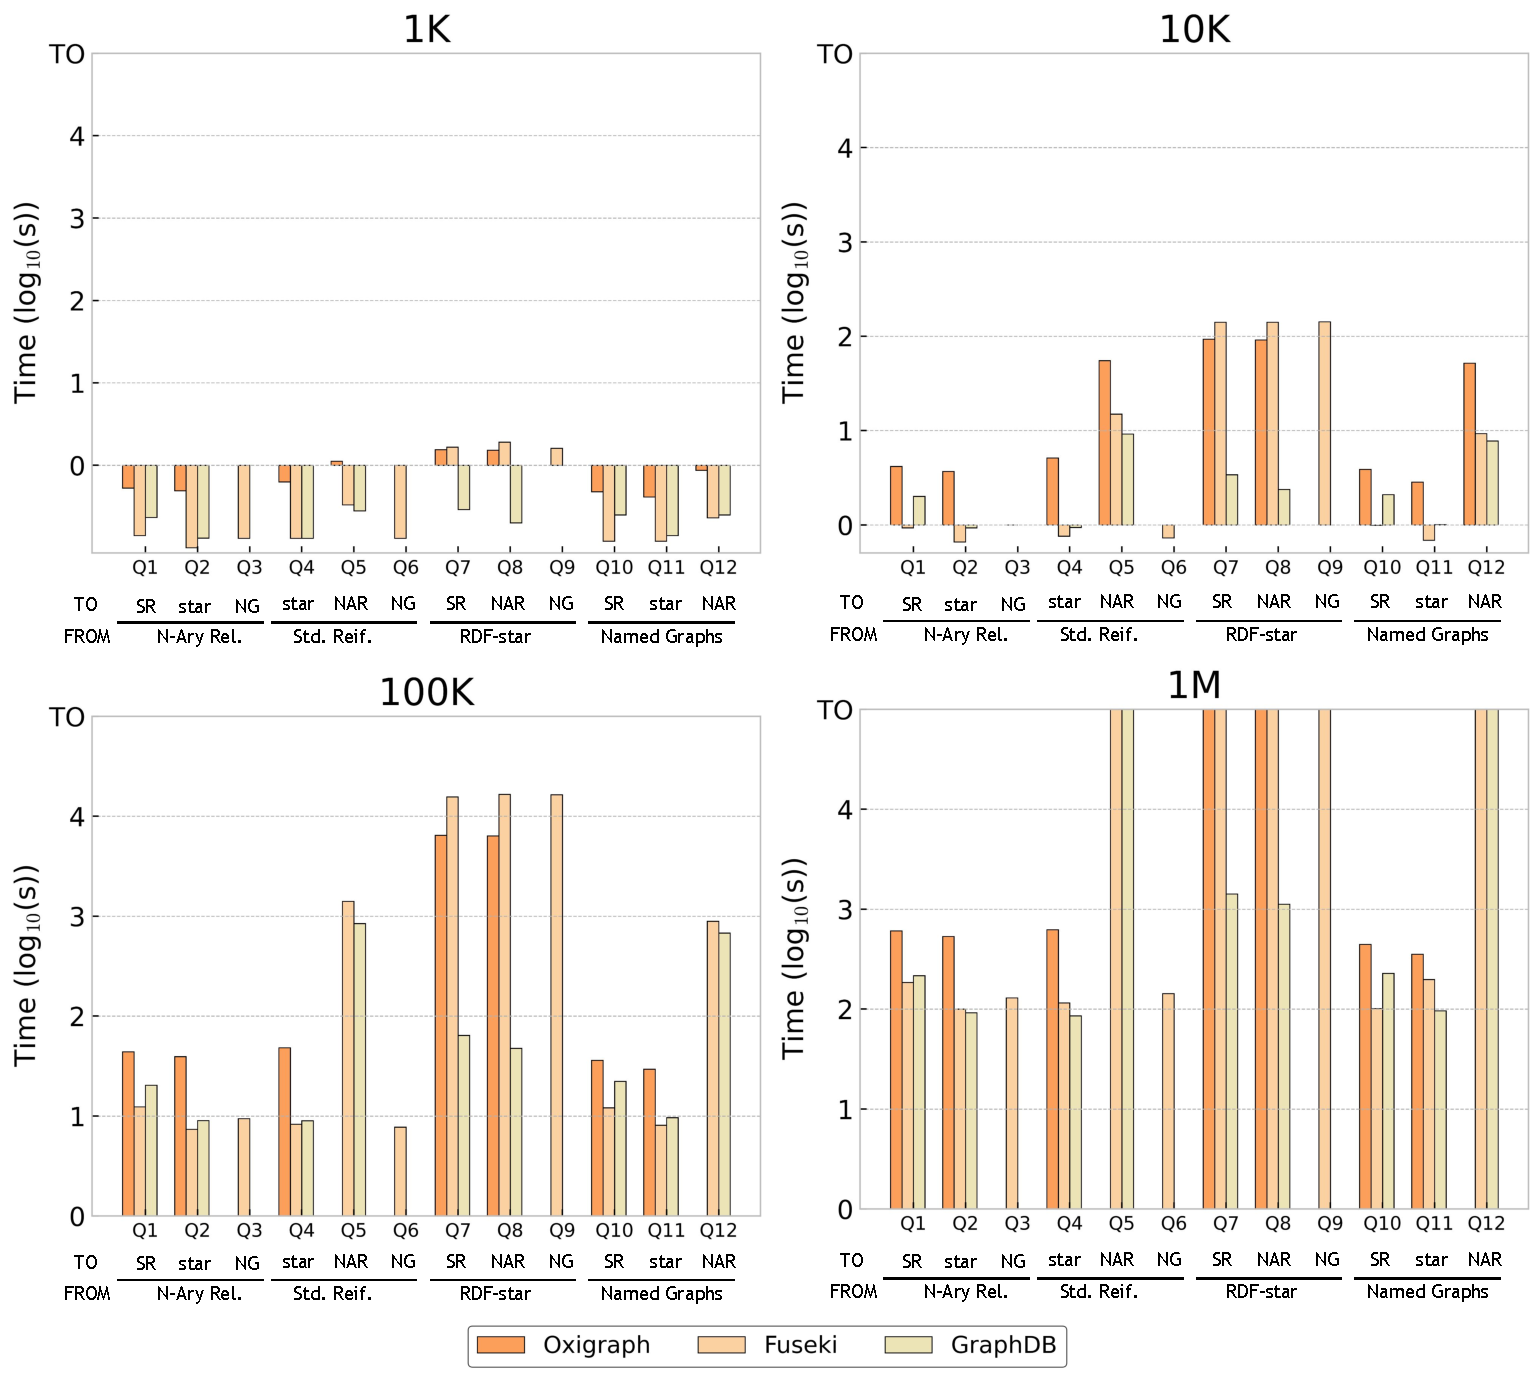
\includegraphics[width=\linewidth]{figures/chp6-1_results-queries.pdf}
    \caption[Execution times of KG re-construction in triplestores]{Execution time of triplestores with the SPARQL queries that perform translations for pairs of representations.}
    \label{fig:chp6-1_queries}
\end{figure}


Looking into the particular differences of the pairs of translation performed with triplestores, we can observe in more detail how the different reification models affect the performance of the graph re-construction with \texttt{CONSTRUCT} queries. \cref{fig:chp6-1_queries} present the results grouping the queries in the legend by the \textit{source} reification representation (i.e. from which representation the dataset is transformed). 

Queries with RDF-star as the source representation (Q7-Q9) generally perform the worst on every scale. This set of queries includes additional SPARQL operators that are usually not required in the rest of queries: \texttt{BIND} and \texttt{FILTER}. Additionally, the recursiveness of the model, together with the fact that it is the only one that makes structural changes over RDF, can produce a negative impact on the performance of the transformation queries. Only GraphDB manages these queries better compared to the other triplestores, reporting better results, while the others reach the time limit in scale 1M. It generates the graph faster than Oxigraph and Fuseki, while it is just slightly slower compared to the queries with other source representations. This may suggest that the additional operators are not the main responsible for the increase of time processing, but the inner performance of the triplestore w.r.t. RDF-star.

The behavior of the construction of N-Ary Relationships is also remarkable. Independently of the source model, it is more costly to produce it than the other models. Queries Q5 and Q12 report an out-of-memory error in Oxigraph for scales 100K and 1M, while reaching timeout in Fuseki and GraphDB in scale 1M. Query Q9 is more affected by the source representation, RDF-star, than the target, thus the result for this query is similar to the ones affected by the abovementioned issue of this model as source. 
Only in GraphDB, Q9 reports less time to produce N-Ary Relationship than Standard Reification, which may be due to having fewer triple patterns to construct (see \cref{tab:chp6-1_query-char}). Interestingly, query Q5 involves an additional operator (\texttt{FILTER}) and more triple patterns than Q4 and Q6, which may explain its low performance. However, query Q12 does not involve any additional operators w.r.t. Q10 and Q11, and has only a few more triple patterns, which does not seem enough justification for its poor performance. Looking at the queries, both Q5 and Q12 contain five joins. Their presence is more likely to be the reason why they take up to two magnitude orders more in the result time than the queries that share source representation. 


%%%%% This one is smaller but visually I think the other (below) is more understandable
%\begin{table}[t!]
%\caption{Geometric mean of the query result times (s) from all triplestores grouping by \textit{source} representation and \textit{target} representation. The lowest times are highlighted in \textbf{bold}, while the highest are %\underline{underlined}.}
%\centering
%\label{tab:closeup-queries}
%\resizebox{\columnwidth}{!}
%{\begin{tabular}{ccccc|cccc}
%    \cmidrule{2-9}
%    & \multicolumn{4}{c|}{\textbf{Source}} & \multicolumn{4}{c}{\textbf{Target}} \\ \midrule
%    \multicolumn{1}{c|}{\textbf{Scale}} & \textbf{Std. Reif.} & \textbf{RDF-star}  & \textbf{N-Graphs} & \textbf{N-Ary Rel.} & \textbf{Std. Reif.} & \textbf{RDF-star}  & \textbf{N-Graphs} & \textbf{N-Ary Rel.} \\ \midrule
%    \multicolumn{1}{c|}{1K} & 0.283 & \underline{0.952} & 0.260 & \textbf{0.204} & 0.387 & \textbf{0.199} & 0.303 & \underline{0.526} \\ \midrule
%    \multicolumn{1}{c|}{10K} & 4.126 & \underline{40.981} & 3.395 & \textbf{1.505} & 5.200 & \textbf{1.366} & 4.693 & \underline{21.218} \\ \midrule
%    \multicolumn{1}{c|}{100K} & 56.612 & \underline{2449.544} & 43.756 & \textbf{16.040} & 154.728 & \textbf{14.066} & 106.176 & \underline{1078.092} \\ \midrule
%    \multicolumn{1}{c|}{1M} & 1085.228 & \underline{15738.107} & 773.737 & \textbf{205.407} & 954.710 & \textbf{180.384} & 927.741 & \underline{28788.048} \\   \bottomrule
%    \end{tabular}}
%\end{table}


%%%% transposed table, occupies more space
\begin{table}[t!]
\caption[Execution time results for re-construction evaluation with triplestores]{Geometric mean of the query result times (s) from all triplestores grouping by \textit{source} representation and \textit{target} representation. The lowest times are highlighted in \textbf{bold}, while the highest are \underline{underlined}.}
\centering
\label{tab:chp6-1_closeup-queries}
\begin{tabular}{cccccc}
    \cmidrule{2-6}
 & \textbf{Representation} & \textbf{1K} & \textbf{10K} & \textbf{100K} & \textbf{1M} \\ \midrule
 \multirow{5}{*}{\textbf{Source}} & \textbf{Std. Reif.} & 0.283 & 4.126 & 56.612 & 1085.228  \\ \cmidrule{2-6}
  & \textbf{RDF-Star} & \underline{0.952} & \underline{40.981} & \underline{2449.544} & \underline{15738.107}  \\ \cmidrule{2-6}
  & \textbf{Named Graphs} & 0.260 & 3.395 & 43.756 & 773.737 \\ \cmidrule{2-6}
 & \textbf{N-Ary Rel.} & \textbf{0.204} & \textbf{1.505} & \textbf{16.040} & \textbf{205.407}  \\ \midrule
 \multirow{5}{*}{\textbf{Target}} & \textbf{Std. Reif.} & 0.387 & 5.200 & 154.728 & 954.710  \\ \cmidrule{2-6}
  & \textbf{RDF-Star} & \textbf{0.199} & \textbf{1.366} & \textbf{14.066} & \textbf{180.384} \\ \cmidrule{2-6}
  & \textbf{Named Graphs}  & 0.303 & 4.693 & 106.176 & 927.741 \\ \cmidrule{2-6}
 \ & \textbf{N-Ary Rel.} & \underline{0.526} & \underline{21.218} & \underline{1078.092} & \underline{28788.048} \\   \bottomrule
\end{tabular}
\end{table}

\cref{tab:chp6-1_closeup-queries} shows a summary of the results from the triplestores grouped by \textit{source} and \textit{target} representation. In general, RDF-star is the fastest representation to construct, while becoming highly inefficient when acting as the source representation. Hence, most of the triplestores do not seem yet optimized to process it. On the contrary, N-Ary relationships perform the fastest being the source representation, but it requires performing joins in the \texttt{CONSTRUCT} that make it the least suitable as a target representation. Standard Reification and Named Graphs perform more consistently overall. Named Graphs take less time than Standard Reification as source and target representation, but can only be generated with Fuseki. 

%Answering \textbf{RQ3}, the combination of representations highly influences the behavior of the triplestores, both in the \texttt{WHERE} and \texttt{CONSTRUCT} clauses. It is especially remarkable for RDF-star and N-Ary Relationships. RDF-star is the fastest representation to generate, but performs the slowest being the source representation; while N-Ary Relationships present the exact opposite behavior. Named Graphs and Standard Reification report a more consistent behavior.




\section{Discussion}
\label{sec:chp6-1_discussion}

This section addresses the following question: given a knowledge graph where reificaiton is needed, is it faster to construct it from the original data sources with the new representation, or to re-construct it within a triplestore?\ana{ojo esta frase, cuadrar con objetivos/RQ cuando estén } To answer this question, we perform an empirical analysis using two KG construction engines and three triplestores, performing the re-construction with four data sizes in four different reification models: RDF-star, Standard Reification, N-Ary Relationships and Named Graphs. Our results show that KG construction engines in general are more scalable, almost independently of the kind of reification. Triplestores perform best for small data sizes. However, their performance is highly dependent on the source representation (in the \texttt{WHERE} clause) and the target representation (in the \texttt{CONSTRUCT} clause). The time for producing RDF-star and Named Graphs is competitive with the KG construction approach. Yet, this approach becomes inefficient for producing N-Ary Relationships due to the need of introducing more joins in the \texttt{CONSTRUCT} clause; and when RDF-star is the source model, since most triplestores are not optimized for its new syntax. 

%%%%%%%%%%%%% SUMMARY AND MAIN CONCLUSIONS %%%%%%%%%%%%
Our evaluation shows that the KG construction engines are more robust for increasing data size and changing the reification models. Performing the re-construction in the triplestore is suitable for small data sizes, but it is largely dependant on the KG structure to offer competitive performance. Thus, we can affirm that performing the re-construction with mappings is in general more reliable, as it is significantly less affected by data size and target representation. 


%%%%%% SPARQL CONSTRUCT rant %%%%%%%
The setup of the evaluation shows us the importance of optimizing SPARQL queries, which gains relevance as the triples to construct increase in number. For instance, the introduction of \texttt{UNION} clauses was needed to avoid costly cartesian products that prevented queries from finishing before the established timeout, or before reaching an out-of-memory error. While this is well known in proficient SPARQL practitioners, it does not come as easily for non-expert users. The performance of SPARQL-Anything, relying almost entirely on SPARQL and Jena processing, is also affected by these different manners of writing the mapping. In contrast, RML mappings are unaffected in this aspect, since how the user writes the mapping does not influence the performance of the compliant systems. SPARQL possess a flexibility and rich expressiveness that languages such as RML lack yet. Nevertheless, it poses the risk for non-expert users to hamper the result retrieval incurring in suboptimal queries. This opens up a challenge for improving the query processing, or even rewriting the queries automatically to be optimized, so as to reduce this accessibility gap for SPARQL.

In addition, this evaluation brings to light that the behavior of the \texttt{CONSTRUCT} clause is not as studied as other SPARQL operators. SPARQL benchmarks often overlook this clause, as it is considered as an extension of \texttt{SELECT}~\citep{schmidt2009sp}. Hence, it is assumed that their performance is comparable and not affected by the change of clause. However, we encountered \texttt{SELECT} queries that returned results in miliseconds, while taking several minutes with \texttt{CONSTRUCT}. 
%% support of GRAPH within CONSTRUCT
%https://stackoverflow.com/questions/59397371/sparql-converting-construct-query-w-named-graph-to-select-query 
This clause also limits the kinds of transformations. For instance, SPARQL 1.1 does not implement generating named graphs (with \texttt{GRAPH}) in \texttt{CONSTRUCT}~\citep{harris2013sparql}.
%\footnote{\url{https://stackoverflow.com/questions/59397371/sparql-converting-construct-query-w-named-graph-to-select-query}}


%%%%%%%%%%% LIMITS OF THE ENGINES %%%%%%%%%%%%
The reported results also open up new challenges for improvement. From the triplestores, only GraphDB could perform reasonably well when RDF-star is the source representation. This highlights the need to continue to improve the processing of this new representation, as it is currently being included in the future RDF 1.2 specification~\citep{hartig2023rdf}. Yet, this representation obtains overall better results when it is the target representation. This will facilitate its adoption, since evolving current KGs into this representation would not suppose an obstacle in terms of performance. 
In addition, all triplestores struggle when the \texttt{CONSTRUCT} clause includes several joins. This fact does not only affect the pairs of transformations studied in this paper, but all potential transformations for evolving knowledge graphs. Regarding KG construction systems, the main challenge still consists of their adoption, as the learning curve for mapping languages is still steep despite efforts to lower it (see \cref{chapter:creation}).


\section{Conclusions}

This chapter addresses the third objective of the thesis \textit{O3: To assess the value of declarative mapping technologies for supporting the evolution of knowledge graphs}.
To this end, we study the re-construction of graphs with different technologies to implement different reification strategies. We evaluate, for a given KG where a change of statement reification is needed, whether it is more efficient to construct the KG from the original data sources with the new representation, or to re-construct it within a triplestore. 
That is, to change the schema of a pre-existing knowledge graph without changing the data. To that end, we perform an empirical analysis using two KG construction engines and three triplestores, performing the re-construction with four data sizes in four different reification models. 
This comprises the main contribution associated with \textit{O3, C6: Identification of scenarios where declarative mapping technologies can support the evolution of knowledge graphs.}
%The results show that KG construction engines in general are more scalable, almost independently of the kind of reification. Triplestores perform best for small data sizes. However, their performance is highly dependent on the source representation (in the \texttt{WHERE} clause) and the target representation (in the \texttt{CONSTRUCT} clause). The time for producing RDF-star and Named Graphs is competitive with the KG construction approach. Yet, this approach becomes inefficient for producing N-Ary Relationships due to the need of introducing more joins in the \texttt{CONSTRUCT} clause; and when RDF-star is the source model, since most triplestores are not optimized for its new syntax. 

%We aim at providing a better understanding of re-constructing knowledge graphs from a reification perspective, contributing to the research on representations interoperability, and how mappings are a key element for scalable transitions. 

